
\documentclass[12pt]{article}
%\setlength{\oddsidemargin}{0in}
%\setlength{\evensidemargin}{0in}
%\setlength{\textwidth}{6.5in}
%\setlength{\parindent}{0in}
%\setlength{\parskip}{\baselineskip}
\thispagestyle{empty}
\usepackage{fullpage}
\usepackage{amsmath,amsthm,amsfonts}
\usepackage{graphicx, graphics}
\usepackage[usenames,dvipsnames]{color}

\definecolor{darkyellow}{rgb}{.929412,.8314,0}
\definecolor{brightgreen}{rgb}{.439,.824,.0863}


\newtheorem*{thm}{Theorem}

\begin{document}

%=======================================================
\begin{center}
{\large \bf Comments for Lecture 12}\\
\bf{2.12.2010}
\end{center}


\noindent {\bf Definition:}  A {\it linear transformation} $T$ from $\mathbb{R}^n$ to $\mathbb{R}^m$ is a function from $\mathbb{R}^n$ to $\mathbb{R}^m$ that must satisfy the following two axioms:

\begin{enumerate}
\item $T({\bf x}+{\bf y})=T({\bf x})+T({\bf y})$ for all ${\bf x}$ and ${\bf y}$ in $\mathbb{R}^n$
\item $T(k{\bf x})=kT({\bf x})$ for all ${\bf x}$ in $\mathbb{R}^n$ and $k$ in $\mathbb{R}$
\end{enumerate}

\noindent {\bf Example 1}:  Let ${\bf x}=\left[ \begin{array}{c} x_1 \\ x_2  \end{array} \right]$ be in $\mathbb{R}^2$ and let $T{:}\mathbb{R}^2 \rightarrow \mathbb{R}$ (remember that $\mathbb{R}$=$\mathbb{R}^1$) be defined as:

\begin{center}
$T({\bf x})=T\left(  \left[ \begin{array}{c} x_1 \\ x_2  \end{array} \right] \right)=x_1+x_2$
\end{center}

To see that $T$ is a linear transformation let's check properties 1. and 2. above:

Let ${\bf x}=\left[ \begin{array}{c} x_1 \\ x_2  \end{array} \right]$ and ${\bf y}=\left[ \begin{array}{c} y_1 \\ y_2  \end{array} \right]$ both be in $\mathbb{R}^2$, and let $k$ be in $\mathbb{R}$.

\begin{enumerate}
\item $T({\bf x}+{\bf y})=T\left(  \left[ \begin{array}{c} x_1 \\ x_2  \end{array} \right]+\left[ \begin{array}{c} y_1 \\ y_2  \end{array} \right] \right)=T\left( \left[ \begin{array}{c} x_1+y_1 \\ x_2+y_2  \end{array} \right]\right)=(x_1+y_1)+(x_2+y_2)=x_1+y_1+x_2+y_2=x_1+x_2+y_1+y_2=(x_1+x_2)+(y_1+y_2)=T\left(  \left[ \begin{array}{c} x_1 \\ x_2  \end{array} \right]\right)+T\left(\left[ \begin{array}{c} y_1 \\ y_2  \end{array} \right] \right)=T({\bf x})+T({\bf y})$
\item $T(k{\bf x})=T\left(k\left[ \begin{array}{c} x_1 \\ x_2  \end{array} \right]\right)=T\left(\left[ \begin{array}{c} kx_1 \\ kx_2  \end{array} \right]\right)=kx_1+kx_2=k(x_1+x_2)=k T\left(  \left[ \begin{array}{c} x_1 \\ x_2  \end{array} \right]\right)=kT({\bf x})$
\end{enumerate}

\noindent So indeed $T$ is a linear transformation from $\mathbb{R}^2$ to $\mathbb{R}$

\noindent {\bf Problem 1}: Let ${\bf x}=\left[ \begin{array}{c} x_1 \\ x_2  \end{array} \right]$ be in $\mathbb{R}^2$ and let $T{:}\mathbb{R}^2 \rightarrow \mathbb{R}^2$ be defined as:

\begin{center}
$T({\bf x})=T\left(  \left[ \begin{array}{c} x_1 \\ x_2  \end{array} \right] \right)=\left[ \begin{array}{c} x_2 \\ x_1  \end{array} \right]$
\end{center}

\noindent Show that $T$ is a linear transformation from $\mathbb{R}^2$ to $\mathbb{R}^2$.

\newpage
\begin{center}
{\Large \bf What in the world did we do today?}
\end{center}
\noindent We actually showed an amazing fact: {\bf Theorem 2.6.1}
\begin{center}
{\Large \bf Say again?}
\end{center}

\noindent So I can give you ANY linear transformation $T$ from $\mathbb{R}^n$ to $\mathbb{R}^m$ and there is a unique $m\times n$ matrix $A$ so that $T({\bf x})=A{\bf x}$ for every ${\bf x}$ in $\mathbb{R}^n$. In fact we know exactly what this matrix is. Column by column we determine the matrix A as:

\[ A = \left[ \begin{array}{cccc} T({\bf e}_1) & T({\bf e}_2) & \ldots & T({\bf e}_n)  \end{array} \right] \]

\noindent (Remember the vectors ${\bf e}_i$ for $1\leq i \leq n$ are the {\it standard basis vectors} see p64)

\begin{center}
{\Large \bf Example!}
\end{center}

\noindent {\bf Example 2}: Consider the linear transformation we have in {\bf problem 1} above.

\noindent Let's find the associated matrix $A$:\\

\noindent Well what will the dimensions of $A$ be (try this yourself)?  The domain of our linear transformation $T$ is $\mathbb{R}^2$ and there are two standard basis vectors in $\mathbb{R}^2$:

\[ {\bf e}_1 = \left[ \begin{array}{c} 1 \\ 0  \end{array} \right] ,\text{ and } {\bf e}_2 = \left[ \begin{array}{c} 0 \\ 1  \end{array} \right]\]

\noindent So from what we have said above we will have:

\[ A = \left[ \begin{array}{cc} T({\bf e}_1) & T({\bf e}_2) \end{array} \right]  \]

\noindent So we actually only need to do two calculations, we need to find both $T({\bf e}_1)$ and $T({\bf e}_2)$.  Well let's do it:

$T({\bf e}_1) = T\left(  \left[ \begin{array}{c} 1 \\ 0  \end{array} \right]\right) = \left[ \begin{array}{c} 0 \\ 1  \end{array} \right] = 1^{\text{st}}$ column of $A$

\noindent and

$T({\bf e}_2) = T\left(  \left[ \begin{array}{c} 0 \\ 1  \end{array} \right]\right) = \left[ \begin{array}{c} 1 \\ 0  \end{array} \right] = 2^{\text{nd}}$ column of $A$

So these are the two columns of $A$ and hence 

\[ A = \left[ \begin{array}{cc} T({\bf e}_1) & T({\bf e}_2) \end{array} \right] =\left[ \begin{array}{cc} 0 &1\\1&0  \end{array} \right]  \]

\noindent So if I gave you a question where you needed to produce the matrix $A$ we would be done.\\

\noindent Well this is interesting.  Remember we are claiming that $T({\bf x})=A{\bf x}$ for every ${\bf x}$ in $\mathbb{R}^n$.  So let's try an example:\\

\noindent Pick your favorite vector in $\mathbb{R}^2$ (the domain).  Since you are not here I will assume it is ${\bf x} = \left[ \begin{array}{c} 3 \\ -4  \end{array} \right]$.  Let's see what happens when $T$ maps this vector to the codomain $\mathbb{R}^2$:

\[ T({\bf x}) =T\left(  \left[ \begin{array}{c} 3 \\ -4  \end{array} \right] \right) = \left[ \begin{array}{c} -4 \\ 3  \end{array} \right]\]

\noindent And now let's see what happens when we find the product $A {\bf x}$:

\[ A{\bf x} = \left[ \begin{array}{cc} 0 &1\\1&0  \end{array} \right] \left[ \begin{array}{c} 3 \\ -4  \end{array} \right] = \left[ \begin{array}{c} -4 \\ 3  \end{array} \right] \] 

\noindent Well that is pretty cool.  And of course this will work for any ${\bf x}$ is $\mathbb{R}^2$, why?  Well we proved that this $A$ is the correct matrix in class (that is what the theorem gives us)!\\

\noindent Just for kicks we could verify that it is indeed true in general:  \\

\noindent Let ${\bf x}=\left[ \begin{array}{c} x_1 \\ x_2  \end{array} \right]$ be in $\mathbb{R}^2$.  Then we have in our example:

\[ A{\bf x} = \left[ \begin{array}{cc} 0 &1\\1&0  \end{array} \right] \left[ \begin{array}{c} x_1 \\ x_2  \end{array} \right] = \left[ \begin{array}{c} x_2 \\ x_1  \end{array} \right] = T({\bf x}). \]

\noindent {\bf Problem 2:}  Find the matrix $A$ associated to the linear transformation in {\bf example 1} above.

\noindent {\bf Problem 3:}  Find the matrix associated to the composition of linear transformations in {\bf example 2} and {\bf example 1}.  Which compositions make sense? 

\noindent {\bf Solution to Exercise (21)5 on page 75:}  This is from Homework 3.  Please attempt this problem on your own before going over the solution:\\

We have a linear transformation $T$ sending each point $(x_1,x_2)$ in the plane $\mathbb{R}^2$ to the point $x_2$ in $\mathbb{R}$.  In other words 
we think of $T$ defined as follows:  For any ${\bf x}=\left[ \begin{array}{c} x_1 \\ x_2  \end{array} \right]$ in $\mathbb{R}^2$ we have

\[ T \left( \left[ \begin{array}{c} x_1 \\ x_2  \end{array} \right] \right)= x_2 \]

We are told $T$ is a linear transformation from $\mathbb{R}^2$ to $\mathbb{R}^1$.  Can you show that?  It is actually very similar to example 1 above.

Now that $T$ is a linear transformation we use the theorem to build the matrix $A$.

What will the dimensions of $A$ be?  Well $T$ is a linear transformation from $\mathbb{R}^2$ to $\mathbb{R}^1$ so $A$ will be a $1\times 2$ matrix.

The theorem says $A = \left[ \begin{array}{cc} T({\bf e}_1) & T({\bf e}_2) \end{array} \right]$ since there are only two standard basis vectors in $\mathbb{R}^2$.

Now find $T({\bf e}_1)$ and $T({\bf e}_2)$.  What did you get?

$T({\bf e}_1) = T\left(  \left[ \begin{array}{c} 1 \\ 0  \end{array} \right]\right) = 0 = 1^{\text{st}}$ column of $A$

$T({\bf e}_2) = T\left(  \left[ \begin{array}{c} 0 \\ 1  \end{array} \right]\right) = 1 = 2^{\text{nd}}$ column of $A$

So this means $A = \left[ \begin{array}{cc} T({\bf e}_1) & T({\bf e}_2) \end{array} \right] = \left[ \begin{array}{cc} 0 & 1 \end{array} \right]$ and this is the answer.  



\noindent {\bf Solution to Exercise (21)1 on page 75:}  This is from Homework 3.  Please attempt this problem on your own before going over the solution:\\

As we discussed in class (and we will do so again in chapter 3) we can actually think of vectors geometrically.

\begin{figure}[h!]
\begin{center} 
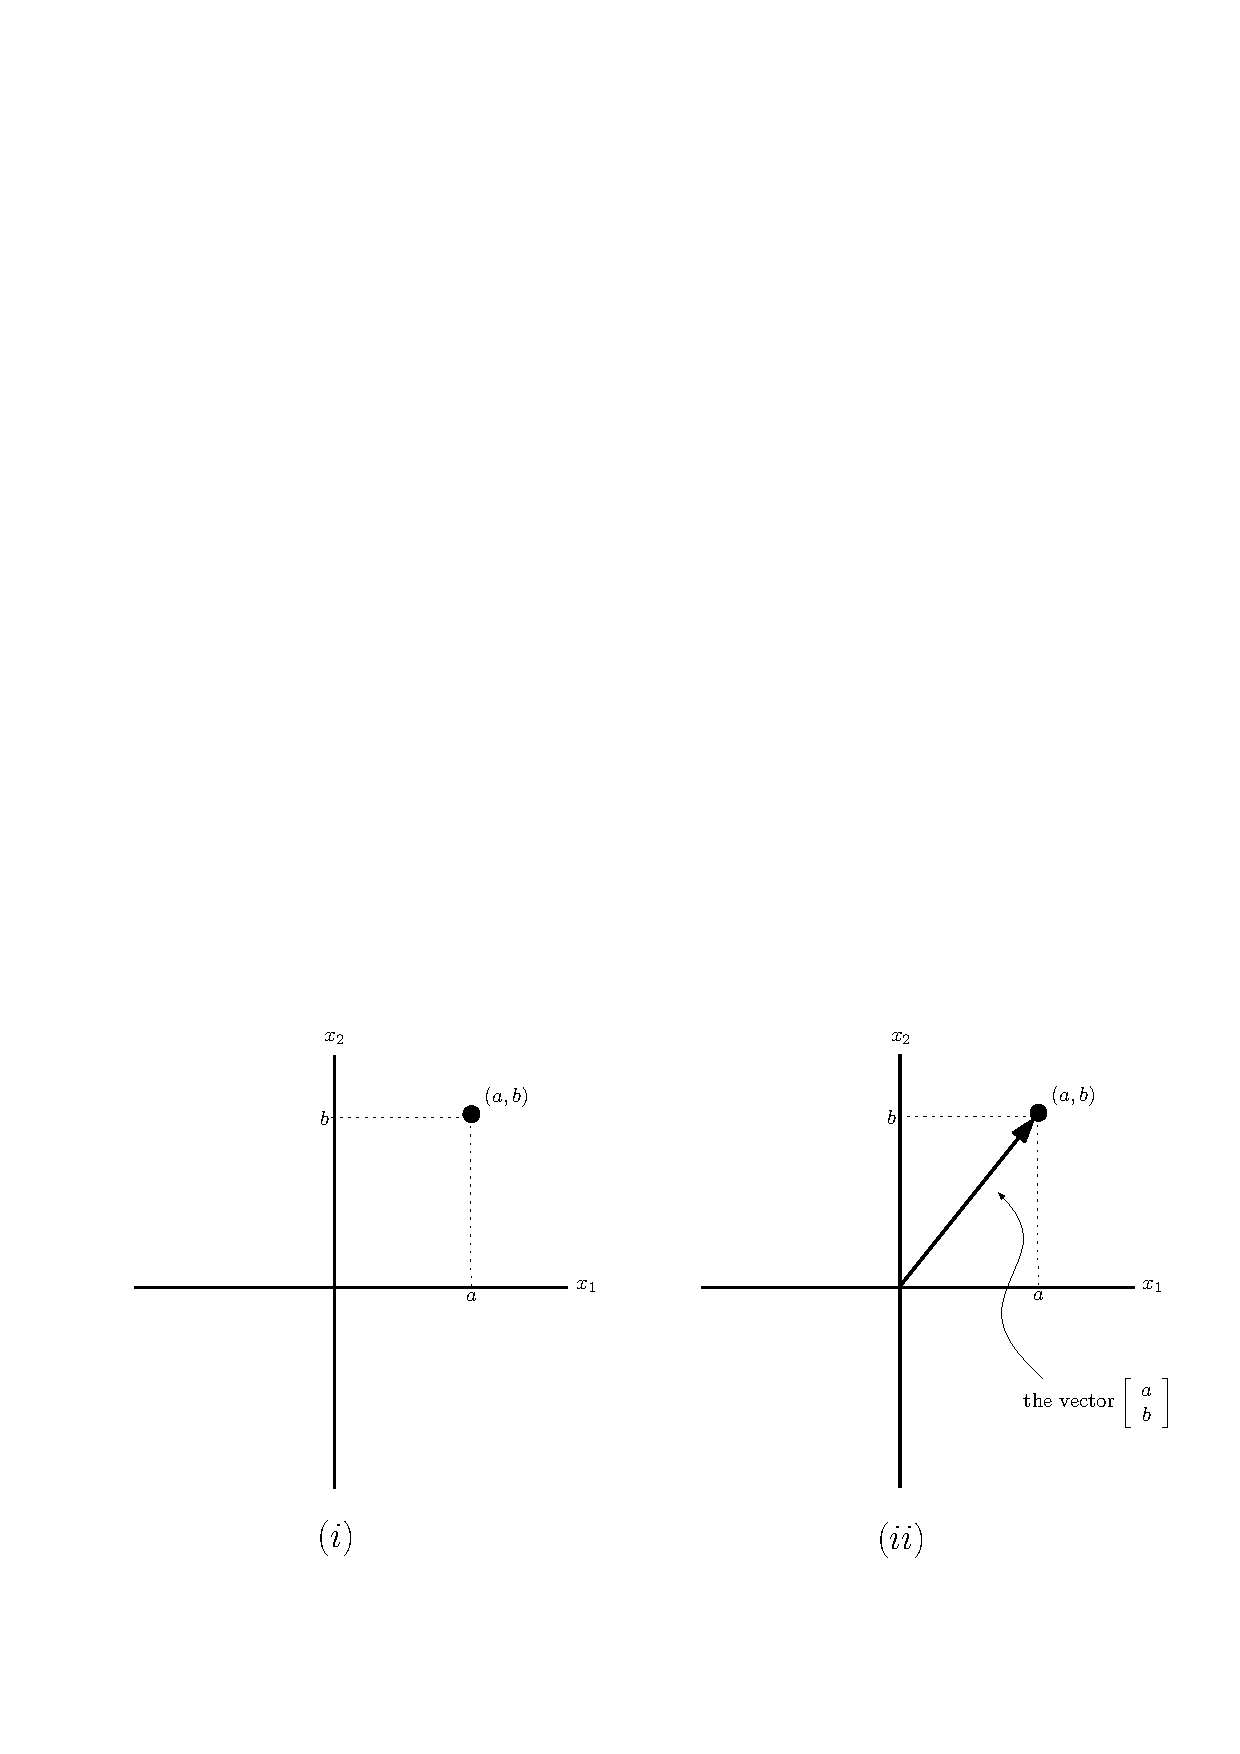
\includegraphics[width = 1 \textwidth]{l12comim1}
\caption{$(i)$ The point $(a,b)$ in $\mathbb{R}^2$, (ii) The point $(a,b)$ and the vector $\left[ \begin{array}{c} a \\ b  \end{array} \right]$ in $\mathbb{R}^2$.}
\end{center}
\end{figure} 

For example, the point $(a,b)$ in $\mathbb{R}^2$, as seen in figure 1(i), has an associated vector $\left[ \begin{array}{c} a \\ b  \end{array} \right]$, as seen in figure 1(ii).  This vector has its tail at the origin (the point $(0,0)$) and its head (noted by the arrow head) at the point $(a,b)$.  This again goes back to our idea of thinking of vectors in $\mathbb{R}^n$ as $n$-tuples representing points of $\mathbb{R}^n$.

Now let's use this geometric interpretation to help us solve the problem.  We need to understand what our linear transformation actually is in order to find the associated matrix from the theorem.

The best part about our theorem is that once we know we have a linear transformation we actually only need to know what it does to the standard basis vectors.

In this particular problem we are told that rotation of the plane $\mathbb{R}^2$ counterclockwise around the origin by 90 degrees is a linear transformation from $\mathbb{R}^2$ to $\mathbb{R}^2$. (NOTE:  in class I actually solved the problem for clockwise rotation).  We need to find the corresponding matrix.

First let's just give this linear transformation the name $T$.  Now let's see where $T$ takes standard basis vectors.  The domain in this problem is again $\mathbb{R}^2$ so there are two calculations: find $T({\bf e}_1)$ and $T({\bf e}_2)$.

Don't forget that $T:\mathbb{R}^2 \to \mathbb{R}^2$ so our outputs will be vectors in $\mathbb{R}^2$.  We see in figure 2 that these output vectors are found by rotating the vectors 90 degrees about the origin. Note that in figure 2 the standard basis vectors ${\bf e}_1$ and ${\bf e}_2$ (the inputs) are drawn as solid black vectors, and the outputs $T({\bf e}_1)$ and $T({\bf e}_2)$ are drawn as dashed red vectors.

\begin{figure}[h!]
\begin{center} 
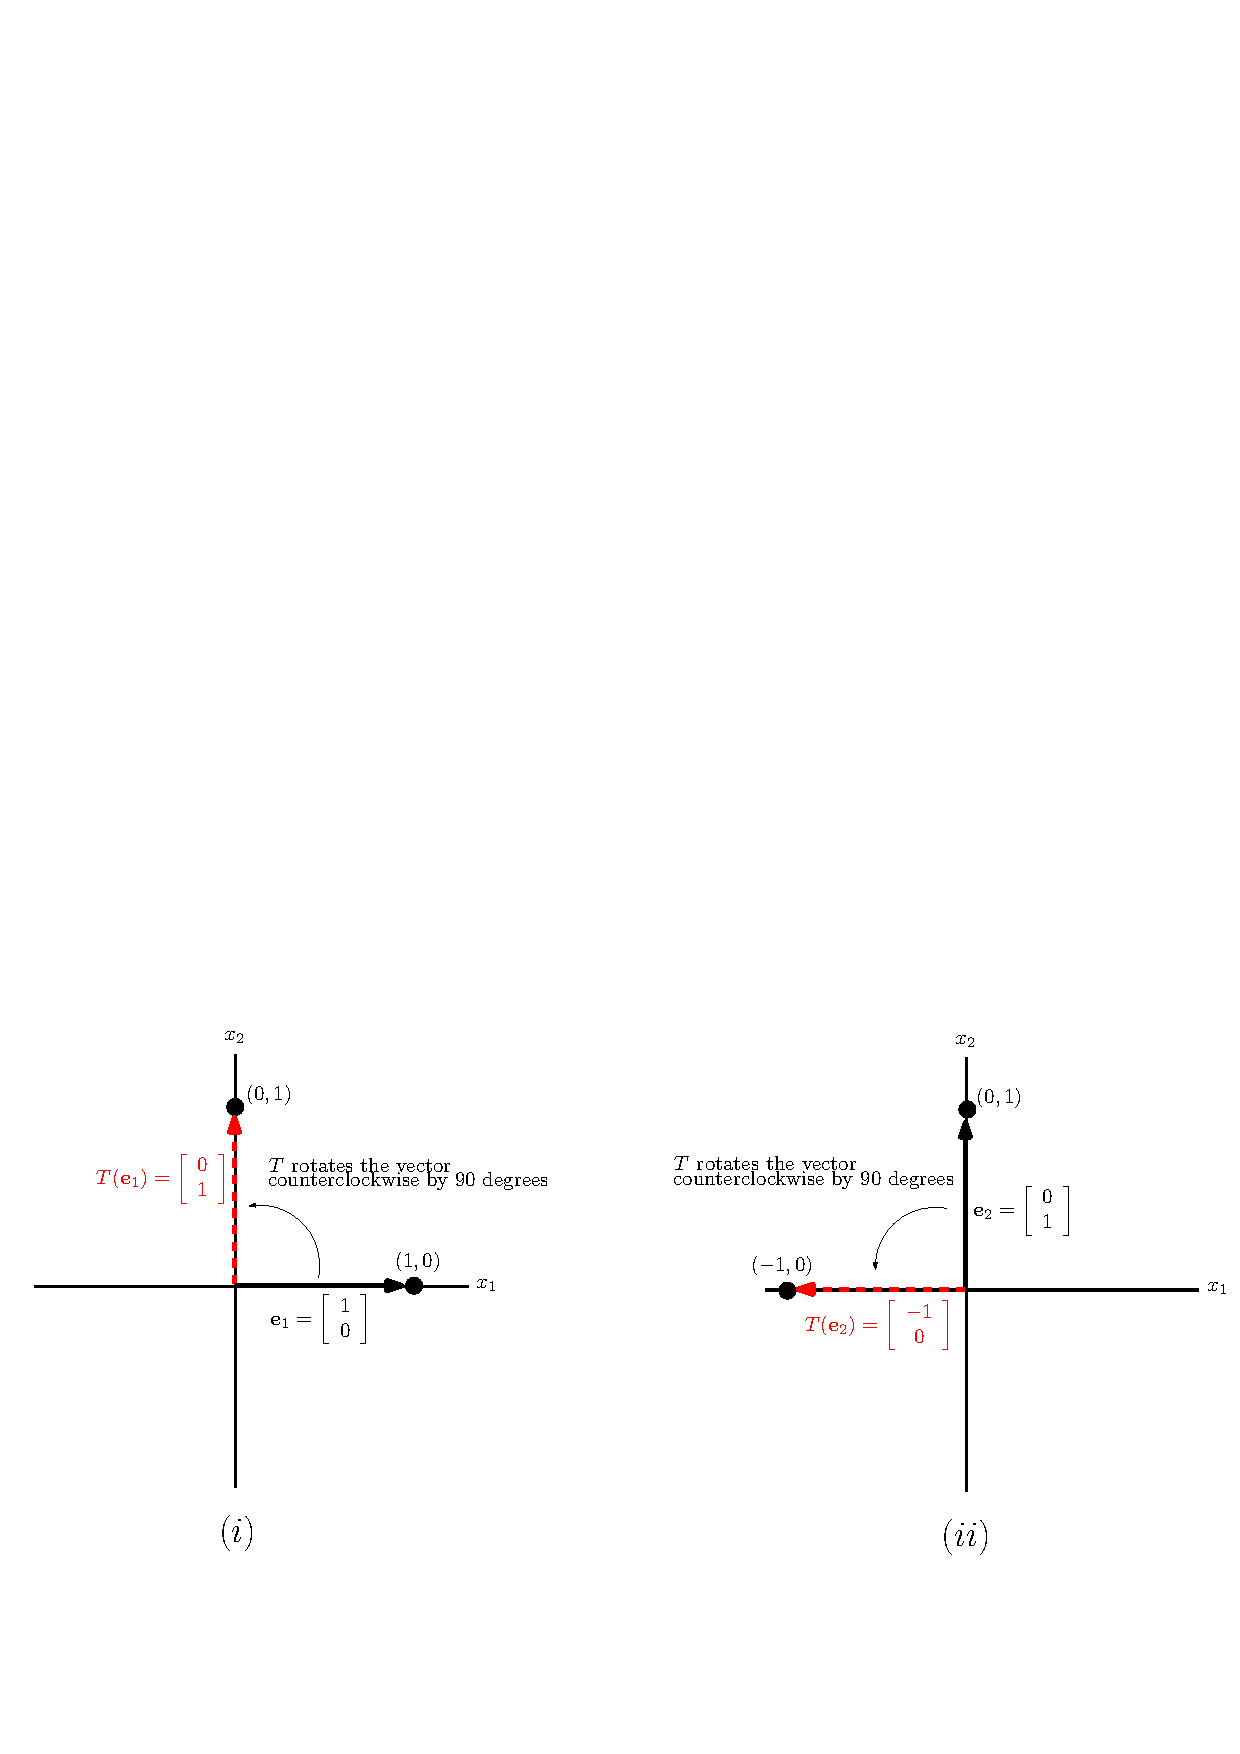
\includegraphics[width = 1 \textwidth]{l12comim2}
\caption{$(i)$ Calculating $T({\bf e}_1)$, (ii) Calculating $T({\bf e}_2)$.}
\end{center}
\end{figure} 

So we have:

$T({\bf e}_1) = T\left(  \left[ \begin{array}{c} 1 \\ 0  \end{array} \right]\right) = \left[ \begin{array}{c} 0 \\ 1  \end{array} \right] = 1^{\text{st}}$ column of $A$

$T({\bf e}_2) = T\left(  \left[ \begin{array}{c} 0 \\ 1  \end{array} \right]\right) = \left[ \begin{array}{c} -1 \\ 0  \end{array} \right] = 2^{\text{nd}}$ column of $A$

So this means $A = \left[ \begin{array}{cc} T({\bf e}_1) & T({\bf e}_2) \end{array} \right] = \left[ \begin{array}{cc} 0 & -1 \\ 1 & 0  \end{array} \right]$ and this is the answer. 



%=======================================================


\end{document}
